% MNRAS manuscript -- compile with: tectonic mnras_a0_lambda_coefficient.tex  (or pdflatex + bibtex + pdflatex x2)
\documentclass[fleqn,usenatbib]{mnras}
\usepackage{newtxtext,newtxmath}
\usepackage[T1]{fontenc}
\usepackage{graphicx}
\usepackage{booktabs}
\usepackage{hyperref}

\title[The coefficient of the $a_0$--$\Lambda$ relation]{The MOND acceleration scale and the cosmological constant: what fixes the coefficient, and the observations that decide it}

\author[C. P. Zimmerman]{Carl P. Zimmerman$^{1}$\thanks{E-mail: to be inserted at submission (see SUBMISSION\_CHECKLIST.md)}
\\
$^{1}$Briar Creek Tech, USA}

\date{Accepted XXX. Received YYY; in original form ZZZ}
\pubyear{2026}

\begin{document}
\sloppy
\label{firstpage}
\pagerange{\pageref{firstpage}--\pageref{lastpage}}
\maketitle

\begin{abstract}
The acceleration scale of the radial-acceleration relation, $a_0$, is numerically close to $\tfrac12 c\sqrt{G\rho_\Lambda}$, where $\rho_\Lambda$ is the dark-energy density. We examine what would fix the coefficient $\kappa$ in $a_0=\kappa c\sqrt{G\rho_\Lambda}$, and what observations can decide it. First, for local relativistic MOND actions on an aether--scalar chassis we show that the additive constant of the MOND primitive is a zero mode of the field equations, degenerate with $\Lambda$ on the cosmological background, so no such action relates $a_0$ to $\Lambda$; the two natural repairs, an empty Newtonian vacuum and a sequestering-type global constraint, fail by sign and by five orders of magnitude. Promoting $a_0$ to the amplitude of a conserved four-form flux makes $a_0\propto\sqrt{G\rho_\Lambda}$ structural and leaves $\kappa$ as a ratio of two couplings; it also predicts an environmental $a_0$ that switches off above $155\,a_0$, invisible in galaxies but shifting the wide-binary boost at 2\,kAU by $-0.02$. Second, we quantify what the data can say. Two estimators on SPARC give $\kappa=0.465\pm0.076$ and $0.551\pm0.043$, both carrying an irreducible dependence on the $H_0$ convention of the distances; the baryonic Tully--Fisher route has a 9.5 per cent mass-budget floor; and at fixed $\Omega_\Lambda$ the prediction scales as $\kappa H_0$, so $\kappa=\tfrac12$ with the Planck $H_0$ and the horizon coefficient $\kappa=\sqrt{8\pi/3}/2\pi=0.461$ with the SH0ES $H_0$ give the same $a_0$ to 0.2 per cent: the coefficient question is degenerate with the $H_0$ tension. Third, we pre-register two tests: the Gaia DR4 wide-binary boost with two mutually exclusive arms and a fixed decision rule, and the deep-MOND Tully--Fisher zero point of a lensed rotator at $z\simeq2.5$, where the prediction is $0.00$ against $+0.33$ dex for a $\Lambda$CDM-native scale.
\end{abstract}

\begin{keywords}
gravitation -- dark energy -- galaxies: kinematics and dynamics -- cosmological parameters -- binaries: visual -- galaxies: high-redshift
\end{keywords}

\section{Introduction}
The radial-acceleration relation of rotationally supported galaxies \citep{McGaugh2016,Lelli2017} is organised by a single acceleration, $a_0\simeq1.2\times10^{-10}$ m s$^{-2}$, whose numerical closeness to $cH_0$ was noted at the birth of MOND \citep{Milgrom1983} and has been read ever since as a hint that the scale is cosmological \citep{SandersMcGaugh2002,FamaeyMcGaugh2012}. Written against the dark-energy density $\rho_\Lambda=\Lambda c^2/8\pi G$ rather than the expansion rate, the coincidence takes the form
\begin{equation}
a_0=\kappa\,c\sqrt{G\rho_\Lambda}=\kappa\,c^2\sqrt{\frac{\Lambda}{8\pi}},\qquad \kappa\simeq\tfrac12,
\label{eq:relation}
\end{equation}
so that $\kappa=\tfrac12$ reads $\Lambda\ell_0^2=32\pi$ with $\ell_0=c^2/a_0$, or in natural units $a_0=M_\Lambda^2/2M_{\rm P}$ with $M_\Lambda^4=\rho_\Lambda$: a seesaw between the vacuum scale and the Planck scale with an exact factor of two. The tie to $\Lambda$ has prior art. \citet{Milgrom1999} derived a MOND-like law from the de Sitter--Unruh temperature and obtained a coefficient corresponding to $a_0=2cH_\Lambda$; entropic re-derivations landed on the same value \citep{Pikhitsa2010,KlinkhamerKopp2011}; \citet{BlanchetLeTiec2009} and \citet{Singh2026} related $a_0$ to $\Lambda$ with coefficients of their own. Relativistic hosts for MOND phenomenology exist, from TeVeS \citep{Bekenstein2004} to the aether--scalar--tensor theory of \citet{SkordisZlosnik2021}, and in all of them $a_0$ and $\Lambda$ are separate parameters.

This paper separates two questions that are often run together. The empirical one, whether $\kappa$ is measured to be near $\tfrac12$ and how well, is answered in Section~\ref{sec:meas} with an honest account of the $H_0$ convention that both available estimators carry. The theoretical one, whether any local action of the aether--scalar class can force the coefficient, is answered in the negative in Section~\ref{sec:theorem}, where we also show what a construction that fixes the sign of the vacuum energy looks like and what it predicts (Section~\ref{sec:fourform}). Section~\ref{sec:data} quantifies what the data can decide, including a degeneracy between the coefficient and the Hubble tension that we have not seen stated elsewhere. Section~\ref{sec:tests} pre-registers the two observations that would move the question: the Gaia DR4 wide-binary boost, for which the programme now carries two mutually exclusive predictions, and the deep-MOND Tully--Fisher zero point at $z\simeq2.5$. We claim neither that equation~(\ref{eq:relation}) is derived nor that its coefficient is; the value of the paper is in stating precisely what is and is not fixed, and by what.

Every number below is produced by a script in the public repository named in the Data Availability section, with checks that can fail; both values of $a_0$ that the programme carries, $9.3619\times10^{-11}$ (from $\rho_\Lambda$ with the Planck parameters) and $1.1279\times10^{-10}$ m s$^{-2}$ (an alternative footing on the total density), are propagated wherever a dimensional number enters.

\section{The relation and its measurement}
\label{sec:meas}
We define $\kappa\equiv a_0/(c\sqrt{G\rho_\Lambda})$ with $\rho_\Lambda=\Omega_\Lambda\,3H_0^2/8\pi G$ evaluated on the Planck 2018 parameters \citep[$H_0=67.4$ km s$^{-1}$ Mpc$^{-1}$, $\Omega_\Lambda=0.685$;][]{Planck2020}, so that $c\sqrt{G\rho_\Lambda}=1.872\times10^{-10}$ m s$^{-2}$ and $\kappa=\tfrac12$ corresponds to $a_0=9.36\times10^{-11}$ m s$^{-2}$. Two estimators on the SPARC sample \citep[175 galaxies, 2803 quality points;][]{Lelli2016} give the measured value.

\emph{The baryonic Tully--Fisher intercept.} In the deep-MOND regime $V_f^4=Ga_0M_b$ \citep{McGaugh2012}, so the intercept of the baryonic Tully--Fisher relation is $a_0$. On SPARC this gives $\kappa=0.465\pm0.076$ (16 per cent). The error is dominated by a mass-budget floor of 9.47 per cent that is independent of sample size, shape assumptions and distances: because $f_*+f_{\rm gas}=1$, the stellar mass-to-light and gas calibrations trade against each other rather than both shrinking, and even perfect distances on the 24 deepest galaxies leave 14.6 per cent. SPARC's Hubble-flow distances assume $H_0=73$ km s$^{-1}$ Mpc$^{-1}$; the Planck-consistent correction is $-3.2$ per cent (the Hubble-flow weight fraction is 0.20, not the 0.58 count fraction), moving the value to 0.450.

\emph{The shape-only estimator.} Under a common rescaling of all distances $g_{\rm bar}=V_{\rm bar}^2/R$ is exactly invariant while $g_{\rm obs}$ rescales, so a fit of the relation's shape with a free vertical offset returns an $a_0$ that is immune to the distance scale; verified on SPARC, it returns the identical $a_0$ at distance rescalings of $0$, $+5$ and $+10$ per cent to five significant figures, and at fixed mass-to-light ratio the statistical-plus-distance budget drops from 6.8 to 1.8 per cent. It gives $\kappa=0.551\pm0.043$ at disc mass-to-light ratios 0.5--0.7. Two caveats apply and we state both. The immunity theorem covers a \emph{common} rescaling; the $H_0$ convention moves only the 97 Hubble-flow galaxies, which sit preferentially at the Newtonian end of the relation (median $g_{\rm bar}=0.33\,a_0$ against $0.18\,a_0$), exactly the lever the shape uses, so re-running with Planck-consistent distances moves the value by $+6.5$ to $+7.3$ per cent, to 0.591, and the self-consistent range is $[0.492,0.591]$. And the disc--bulge mass-to-light degeneracy is relocated rather than broken: across the bulge mass-to-light range the estimate spans $0.41$--$0.60$.

The structural point, established in the repository's convention audit, is that $\kappa\propto h^{2q_{\rm eff}-p}$ with $p=1$ (or $1/\Omega_\Lambda$) from the denominator and $q_{\rm eff}$ the estimator's effective distance exponent ($+0.20$ for the intercept, $-0.41$ for the shape-only estimator): no estimator on present data is $H_0$-invariant, and $\kappa$ must be quoted with the $H_0$ it was computed at. Fig.~\ref{fig:kappa}(a) shows both measurements with their convention ranges against the candidate coefficients of Table~\ref{tab:cands}. Four simple candidates lie within $2\sigma$ of the measurements; the data do not single out $\tfrac12$.

\begin{table}
\caption{Candidate coefficients in $a_0=\kappa c\sqrt{G\rho_\Lambda}$ and their pulls against the two SPARC estimators (Planck $H_0$ convention): the intercept value $0.465\pm0.076$ and the shape-only value $0.551\pm0.043$. The last two rows are the de Sitter--Unruh derivations of the coefficient, which are excluded.}
\label{tab:cands}
\begin{tabular}{lccc}
\toprule
coefficient & $\kappa$ & pull (int.) & pull (shape)\\
\midrule
$c^2/(2\pi L_{\rm dS})$, horizon form & 0.461 & $0.1\sigma$ & $2.1\sigma$\\
$\tfrac12$, this programme's target & 0.500 & $0.5\sigma$ & $1.2\sigma$\\
$cH_0/2\pi$, the original coincidence & 0.557 & $1.2\sigma$ & $0.1\sigma$\\
$1/\sqrt3$ & 0.577 & $1.5\sigma$ & $0.6\sigma$\\
$\sqrt{3/8}$ & 0.612 & $1.9\sigma$ & $1.4\sigma$\\
$a_0=cH_\Lambda$ & 2.89 & excl. & excl.\\
$a_0=2cH_\Lambda$ \citep{Milgrom1999} & 5.79 & excl. & excl.\\
\bottomrule
\end{tabular}
\end{table}

\begin{figure*}
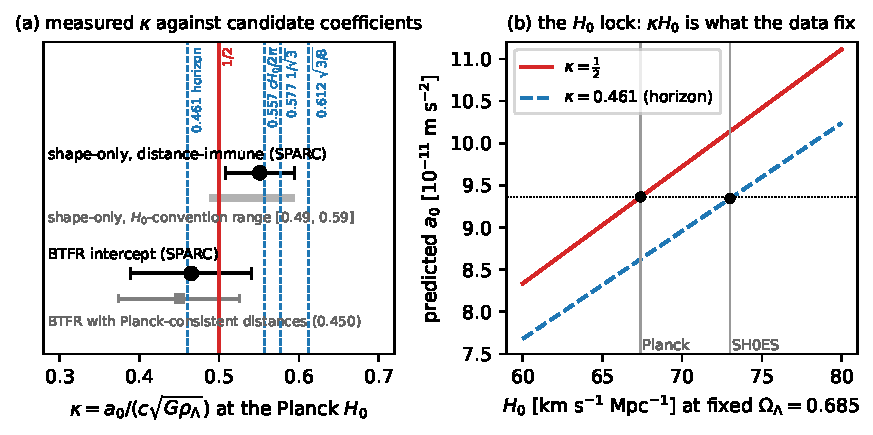
\includegraphics[width=\textwidth]{fig1_kappa_h0.pdf}
\caption{(a) The two SPARC determinations of $\kappa$ (black), their $H_0$-convention shifts (grey: the intercept with Planck-consistent distances; the shape-only estimator's self-consistent range), and the candidate coefficients of Table~\ref{tab:cands} (vertical lines; the frozen $\tfrac12$ in red). (b) The $H_0$ lock: at fixed $\Omega_\Lambda$ the predicted $a_0$ scales as $\kappa H_0$, so $\kappa=\tfrac12$ on the Planck $H_0$ and $\kappa=0.461$ on the SH0ES $H_0$ predict the same $a_0$ to 0.2 per cent (black points on the dotted line). Script: \texttt{make\_figures.py}, from \texttt{kappa\_closure/k03}.}
\label{fig:kappa}
\end{figure*}

\section{No local action of the aether--scalar class fixes the coefficient}
\label{sec:theorem}
\subsection{The action class}
We work with the class of actions that host MOND phenomenology on a preferred-frame chassis: an Einstein--aether or khronometric sector \citep{JacobsonMattingly2001,Blas2011} supplying a unit timelike vector $n_\mu$, a scalar $\phi$ whose spatial gradient $Y=q^{\mu\nu}\partial_\mu\phi\partial_\nu\phi$ carries the MOND non-linearity through a primitive $J(Y)$, and an explicit cosmological constant. The aether--scalar--tensor theory of \citet{SkordisZlosnik2021} is the best-known member; the programme's own candidate \citep{Zimmerman2026filtered,Zimmerman2026ceiling} is the khronometric member
\begin{equation}
\begin{split}
S=\int d^4x\sqrt{-g}\,\frac{1}{16\pi G}\Big[R-2\Lambda-\sum_i c_iT_i+2(2-K_B)J^\mu\partial_\mu\phi\\
-K(Q)-(2-K_B)J(Y)\Big]+S_m,
\end{split}
\label{eq:action}
\end{equation}
with $J^\mu=n^\nu\nabla_\nu n^\mu$ the aether acceleration, $Q=n\cdot\partial\phi$, $K=K_2(Q-Q_0)^2$, $c_1=-c_3=K_B$, the $T_i$ the standard aether invariants, and a coherence operator $\xi^2|\nabla_\perp V|^2$ carried inside the argument of $J$ that screens the Solar System \citep{Zimmerman2026filtered}. The kernel enters every equation through one function $J_Y(s)=s/\Delta(s)$, where the scalar's boost is $g_\phi=a_0\Delta(s)$ at Newtonian acceleration $g_N=sa_0$; the carried kernel is the radial-acceleration function, $\Delta=s/(e^{\sqrt s}-1)$, saturated at its maximum $s_{\rm sat}=2.540$, $\Delta_{\rm sat}=0.6476$, because a bounded boost must be single-valued \citep{Zimmerman2026ceiling}. In units of $a_0^2$ the primitive is $j(s)=2\int_0^s s'\,d\Delta$, with $j(s_{\rm sat})\equiv I=0.4525$.

\subsection{The zero mode}
The static field equations of equation~(\ref{eq:action}) contain $J$ only through $J'$: the scalar equation is $\nabla\!\cdot\!(J_Y\nabla\phi)=\nabla^2\Psi$ for any $J$, so $J\to J+C$ is a symmetry of the local sector. On the FLRW background, where $Y=0$ and $Q=Q_0$, the constant part of the minisuperspace Lagrangian is $-a^3[2\Lambda+(2-K_B)J(0)+K(Q_0)]$, so the background sees only
\begin{equation}
\Lambda_{\rm eff}=\Lambda+\tfrac12(2-K_B)J(0)+\tfrac12K(Q_0).
\end{equation}
With $\Lambda$ explicit and free, no equation of the action relates $a_0$ to $\Lambda$. This is elementary, and we state it as a theorem only because the programme's own literature, and some of the entropic derivations, have implicitly assumed otherwise: an interpolation law fixes derivatives of the primitive, while $\rho_\Lambda$ reads its additive zero, and those are independent data. Both steps are executed symbolically in the script \texttt{k01}.

\subsection{Repair 1: the $\Lambda$-free vacuum}
Delete the explicit $\Lambda$ and fix the zero of the primitive by the only principle available to a local action, an empty Newtonian vacuum ($J=0$ at the saturated end). The background then carries $\rho_{\rm vac}=(2-K_B)J(0)/16\pi G=-(2-K_B)Ia_0^2/16\pi G$. Its sign is negative for every kernel of the class, because the scalar's gradient term must be attractive for the scalar to boost gravity at all, and its primitive therefore rises toward the Newtonian end. Its size is $|\rho_{\rm vac}|/\rho_\Lambda=(2-K_B)I\kappa^2/16\pi=0.0045$ for the carried kernel (0.0007 for the exponential carrier), against a required $|J(0)|=16\pi a_0^2/((2-K_B)\kappa^2)=100\,a_0^2$, a factor 220 above the primitive's whole span. The constant $4\pi^4/15$ of the radial-acceleration primitive, which would give $\kappa=\sqrt{60/((2-K_B)\pi^3)}=0.98$--$1.05$ if read as the vacuum energy, is what the unsaturated, non-monotone branch returns ($2\int_0^\infty s\,d\Delta=-4\pi^4/15$), the branch the bounded-boost requirement forbids; the coefficient that would put it at $\tfrac12$ is 7.7 against the action's $2-K_B\le2$, and no term supplies it.

\subsection{Repair 2: a global constraint}
The one class of principle that removes an additive zero mode without choosing a constant is a global constraint of the vacuum-energy-sequestering type \citep{KaloperPadilla2014}, in which $\Lambda$ becomes a Lagrange multiplier fixed by the spacetime average of the field Lagrangians. The only sector with scale $a_0^2$ is the scalar, whose on-shell, curl-free Lagrangian density is pointwise $(2-K_B)a_0^2F(s)/16\pi G$ with $F=2s\Delta-j$ ($\to\tfrac43s^{3/2}$ in deep MOND). Averaged over the cosmic peculiar-acceleration field, Maxwellian with rms $0.005$--$0.012\,a_0$ today for $v_{\rm rms}=300$--$600$ km s$^{-1}$ and scaling as $D(a)/a^2$, the ratio $\langle L_\phi\rangle/\rho_\Lambda$ is $0.6$--$2.3\times10^{-5}$ today, falls to $10^{-8}$ of that when the average is extended to $10t_0$ because the de Sitter future dominates the volume, and would reach unity only for a universe sitting at $54$--$89\,a_0$ on average. A halo term at a hundred times its filling factor changes nothing. The route is closed on magnitude, independently of sign and of the $O(1)$ convention (script \texttt{k02}).

Taken together: the additive zero of the primitive cannot be fixed inside the scalar sector, the sign cannot be flipped there without a ghost, and the magnitude $\rho_\Lambda c^2=4a_0^2/G$ that $\kappa=\tfrac12$ requires is an $O(1)$ multiple of $a_0^2/G$ with no $16\pi$, which places any successful principle in the geometric or boundary sector. The coefficient is, for this class, an empirical boundary condition.

\section{A four-form construction: structure for the form, a coupling ratio for the coefficient}
\label{sec:fourform}
A three-form gauge potential with four-form field strength $F_{\mu\nu\rho\sigma}=q\,\epsilon_{\mu\nu\rho\sigma}$ carries vacuum energy without propagating modes \citep{DuffvanNieuwenhuizen1980,BoussoPolchinski2000}. For a vacuum action $P(q)$ the gravitating energy is the Legendre form $\varepsilon=qP_q-P$ rather than $-P$, because $q$ depends on the metric through the volume element. Promote the MOND scale to the flux, $a_0=\beta\sqrt G|q|$, with $P=Zq^2/2$. The primitive's constant becomes $b\beta^2q^2$ with $b=(2-K_B)I/16\pi$, its gravitating energy is $+ba_0^2/G$, and the sign of Section~\ref{sec:theorem} is reversed without touching the attractive gradient term. Both $a_0$ and $\rho_\Lambda$ are now set by one conserved flux, so $a_0\propto\sqrt{G\rho_\Lambda}$ is structural and the flux amplitude cancels:
\begin{equation}
\kappa^2=\frac{a_0^2}{G\varepsilon_{\rm vac}}=\frac{2\beta^2}{Z+2b\beta^2},\qquad \kappa=\tfrac12\iff Z/\beta^2=8-2b=7.96.
\label{eq:fourform}
\end{equation}
The coefficient has become a ratio of two couplings that nothing in the construction fixes; the question ``why $32\pi$'' has become ``why $Z=8\beta^2$''.

The promotion has a consequence that must be computed rather than inherited. Since $J$ depends on $a_0$, the four-form equation $\partial_\mu(\partial\mathcal L/\partial q)=0$ reads $q[Z+(2-K_B)\beta^2(s\Delta-j)/8\pi]=Zq_0$, with $\partial J/\partial a_0|_Y=(2/a_0)(J-YJ_Y)$ and $YJ_Y=g_\phi g_N$. In the saturated regime the equation is linear in $q$, giving
\begin{equation}
a_0^{\rm loc}=a_0\Big(1-\frac{g_N}{g_*}\Big),\qquad g_*=\frac{8\pi Z a_0}{(2-K_B)\beta^2\Delta_{\rm sat}}=155\,a_0 ,
\end{equation}
and above $g_*=1.4\times10^{-8}$ m s$^{-2}$ the only solution is $q=0$: the scalar switches off (Fig.~\ref{fig:fourform}a). The environmental $a_0$ is 1.2 per cent low at the knee of the radial-acceleration relation and 64 per cent low at $100\,a_0$, yet the relation moves by less than 0.002 dex because the boost is already a small fraction of $g_N$ there. Inside 205 AU of the Sun the scalar is off, so the planetary monopole residual vanishes without the coherence length; the Cassini quadrupole \citep{Bertotti2003,Hees2016} is set near $s\approx1$ where $a_0^{\rm loc}=0.997a_0$, so the coherence length is still required. For a $1.5M_\odot$ wide binary $a_0$ is 15 per cent low at 2\,kAU, which shifts the innermost Gaia DR4 bin of the boost by $\delta\gamma_v=-0.019$ (canonical) or $-0.015$ (alternative footing), about one sigma at the frozen error model (Fig.~\ref{fig:fourform}b). The construction is recorded as a variant in the pre-registration of Section~\ref{sec:dr4}, not as a registered number.

\begin{figure*}
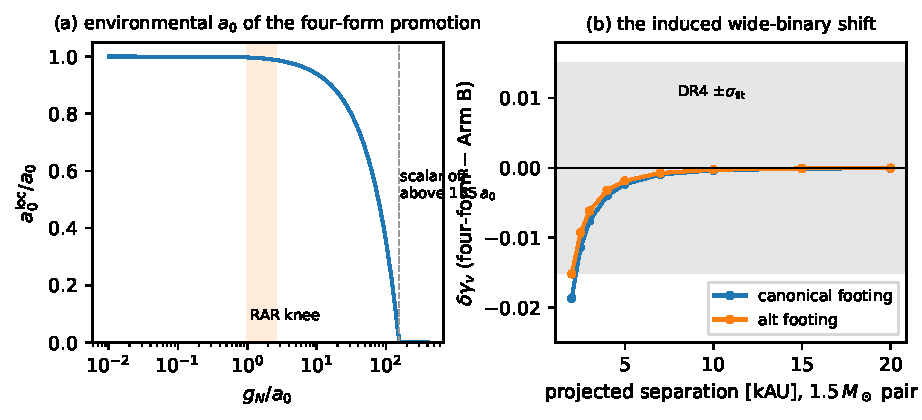
\includegraphics[width=\textwidth]{fig2_fourform.pdf}
\caption{The four-form promotion $a_0=\beta\sqrt G|q|$ at $Z=8\beta^2$. (a) The environmental scale $a_0^{\rm loc}/a_0$ against $g_N/a_0$: 1.2 per cent low at the radial-acceleration knee (shaded), linear to zero at $155\,a_0$, and off beyond. (b) The induced shift of the wide-binary velocity boost for a $1.5M_\odot$ pair on both $a_0$ footings, against Gaia DR4's frozen $\sigma_{\rm fit}=0.019$ (grey band). Script: \texttt{make\_figures.py}, from \texttt{kappa\_closure/k04}.}
\label{fig:fourform}
\end{figure*}

\section{What the data can decide}
\label{sec:data}
\subsection{Separating the candidates}
Section~\ref{sec:theorem} leaves one coefficient-free identification with the right sign and size, the horizon form $a_0=c^2/(2\pi L_{\rm dS})$, i.e.\ $\kappa=\sqrt{8\pi/3}/2\pi=0.4607$. (This is not the \citet{Milgrom1999} construction, which fixes $a_0=2cH_\Lambda$ and is excluded.) It differs from $\tfrac12$ by 8.5 per cent in $a_0$, $0.036$ dex. A $3\sigma$ separation needs 2.8 per cent on $a_0$; the intercept route carries the 9.5 per cent floor of Section~\ref{sec:meas}, a factor 3.3 short and a floor rather than a statistics limit, and the shape-only estimator's convention range alone spans 20 per cent. The Gaia DR4 wide-binary boost has $d\ln\gamma_v/d\ln a_0=0.1155$ and returns $a_0$ to 21 per cent; it cannot contribute. Combining the two measurements, $\ln[L(\tfrac12)/L(0.461)]=+1.4$: undecided.

\subsection{The $H_0$ lock}
At fixed $\Omega_\Lambda$ the prediction of equation~(\ref{eq:relation}) scales as $\kappa H_0$. Hence $\kappa=\tfrac12$ on the Planck $H_0=67.4$ and $\kappa=0.461$ on the SH0ES $H_0=73.0$ km s$^{-1}$ Mpc$^{-1}$ \citep{Riess2022} predict the same $a_0$ to 0.2 per cent (Fig.~\ref{fig:kappa}b): the ratio $0.461/0.5=0.921$ equals $67.4/73.0=0.923$. The coefficient question is therefore numerically the Hubble tension. Holding $\Omega_mh^2$ to the CMB value instead of $\Omega_\Lambda$ puts the SH0ES reading at $0.447$, 3 per cent from the horizon form. Run the other way, a frozen $\kappa=\tfrac12$ turns $a_0$ into an $H_0$ meter: the shape-only $a_0$ gives $H_0=74\pm6$ and the intercept $a_0$ gives $63\pm10$ km s$^{-1}$ Mpc$^{-1}$, straddling the tension. Two consequences follow. A statement that the coefficient is exactly $\tfrac12$ has always quietly committed to the Planck $H_0$ and to a distance scale for the galaxies, and it should say so. And a resolution of $H_0$ would tell us which coefficient the measured $a_0$ corresponds to, but only at the 8 per cent level, below the floor on $a_0$ itself, so it would separate $\tfrac12$ from 0.461 at about $1\sigma$. The coefficient is a precision problem gated by the stellar mass-to-light zero point, the absolute gas scale and $H_0$.

\section{Two pre-registered tests}
\label{sec:tests}
\subsection{The Gaia DR4 wide-binary boost: two mutually exclusive arms}
\label{sec:dr4}
Wide binaries at 2--30 kAU probe accelerations near $a_0$ with no dark matter and are the sharpest local test of the external-field-dominated MOND regime; Gaia DR3 analyses disagree on whether a boost is present \citep{Chae2023,Banik2024}, largely on sample purity. The programme froze a pre-registration before the data \citep{Zimmerman2026prereg}: a fixed estimator (median $\tilde v=v_\perp/v_{\rm circ}$ in bins of $y=g_N/a_0$ against a noise-convolved Newtonian forward model, one-parameter deep asymptote $\gamma_v$, a profiled eccentricity nuisance), a frozen cut table on the El-Badry catalogue conventions \citep{ElBadry2021}, the DR4 error model scaled from EDR3 \citep{Lindegren2021}, $N=30\,000$ pairs, $\sigma_{\rm fit}=0.019$ and $\sigma_{\rm tot}=0.028$, and a reporting rule that emits raw $\hat\gamma_v$ with its distances to every registered anchor and never a verdict word. The analysis has been re-run end to end on the DR3-era catalogue (10\,624 pairs after the frozen cuts; $\hat\gamma_v=1.2075\pm0.035$ on both footings, contaminated by the missing triple and faint-companion screens and non-scoring by the pre-registration's own rule).

The programme now carries two mutually exclusive predictions, both registered in Amendment 11 of the pre-registration before DR4 (Table~\ref{tab:dr4}, Fig.~\ref{fig:dr4}). Arm A is the frozen kernel as modified gravity with no coherence length, the full non-linear AQUAL-EFE solve giving the band $\gamma_v=1.1614$--$1.1814$ (canonical) and $1.1917$--$1.2267$ (alternative footing). Arm B is the covariant candidate of equation~(\ref{eq:action}) at the smallest coherence length that passes the Cassini quadrupole ($\xi\ge0.10$ pc canonical, 0.15 pc alternative), evaluated with the same estimator; because the coherence length lowers the boost, its numbers are ceilings: $\gamma_v\le1.0450$ and $\le1.0300$, falling toward Newton as $\xi$ grows. The arms exclude each other because Arm A's kernel as strict AQUAL fails the Cassini quadrupole by a factor 4--5, and with the length that passes Cassini it is Arm B. The decision rule is fixed in advance (Table~\ref{tab:dr4}). Stated against interest: DR4 separates the arms at $4.2\sigma_{\rm tot}$ but cannot confirm Arm B over Newton beyond $1.6\sigma_{\rm tot}$ even if the truth sits at its ceiling; a Newtonian result falsifies Arm A and leaves Arm B alive but unconfirmed, and the pre-registration forbids describing that outcome as a success.

\begin{table}
\caption{The Gaia DR4 decision rule (Amendment 11; $\sigma_{\rm tot}=0.028$, canonical footing; alternative footing shifted correspondingly). Newton is $\gamma_v=1.000$.}
\label{tab:dr4}
\begin{tabular}{lll}
\toprule
$\hat\gamma_v$ lands in & Arm A & Arm B\\
\midrule
$\le1.007$ & falsified ($\ge5.5\sigma$) & alive only as its Newtonian limit\\
$1.007$--$1.056$ & falsified ($\ge3.8\sigma$) & consistent; not separable from Newton\\
$1.056$--$1.084$ & disfavoured (2.8--3.8$\sigma$) & consistent; Newton disfavoured 2--3$\sigma$\\
$1.084$--$1.101$ & 2.2--2.8$\sigma$ below floor & within $2\sigma$ of ceiling: arm undecided\\
$1.101$--$1.129$ & within $2.2\sigma$ of floor & disfavoured (2--3$\sigma$)\\
$\ge1.129$ & scoreable (Amendment 10) & falsified ($>3\sigma$ above ceiling)\\
$>1.23$ & no-verdict edge & falsified\\
\bottomrule
\end{tabular}
\end{table}

\begin{figure*}
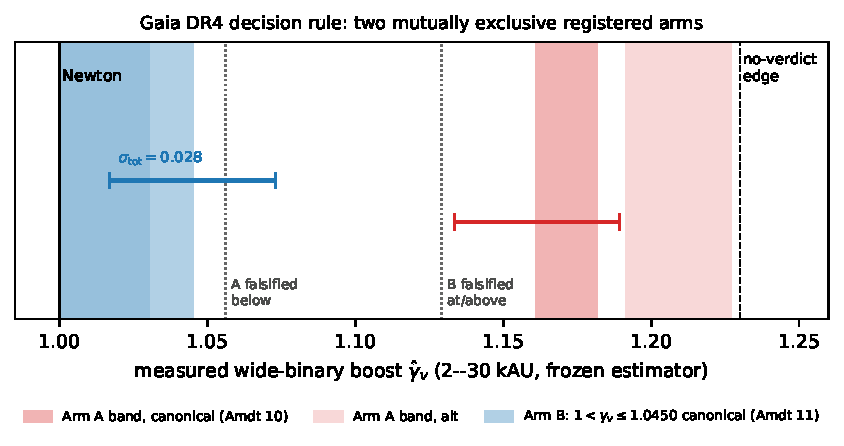
\includegraphics[width=\textwidth]{fig3_dr4_rule.pdf}
\caption{The two registered wide-binary arms and the fixed decision rule of Table~\ref{tab:dr4}. Red: Arm A's computed bands (Amendment 10). Blue: Arm B's ceilings (Amendment 11), the covariant candidate predicting $1<\gamma_v\le$ ceiling. Error bars show $\sigma_{\rm tot}=0.028$ at the frozen $N=30\,000$. Script: \texttt{make\_figures.py}.}
\label{fig:dr4}
\end{figure*}

\subsection{The deep-MOND Tully--Fisher zero point at $z\simeq2.5$}
\label{sec:a0z}
Equation~(\ref{eq:relation}) predicts $a_0(z)/a_0(0)=\sqrt{\rho_{\rm DE}(z)/\rho_{\rm DE}(0)}$: flat for a cosmological constant, and $0.82$ at $z=2.5$ on the DESI DR2 $w_0w_a$ fit. In deep MOND $V_f^4=Ga_0M_b$, so the baryonic Tully--Fisher zero point at fixed velocity moves by $\Delta_{\rm BTFR}=-\log_{10}[a_0(z)/a_0(0)]$: $0.00$ dex ($-0.09$ with DESI dark energy). $\Lambda$CDM has no fundamental $a_0$; its emergent radial-acceleration scale rises with the halo structure, $a_s\propto E(z)^{4/3}c^2/f(c)$ with $f(c)=\ln(1+c)-c/(1+c)$, by a factor 2.13 at $z=2.5$ for the \citet{DuttonMaccio2014} concentrations at $10^{12}M_\odot$ (2.80 for \citealt{Duffy2008}; 3.17 for the Magneticum apparent rise), i.e.\ $\Delta_{\rm BTFR}\simeq+0.33$ dex or 20 per cent in velocity at fixed mass (Fig.~\ref{fig:a0z}). One point with total uncertainty $0.13$ dex separates the two at 20:1.

The existing archives cannot decide this. A joint likelihood over twelve published constraints \citep[among them][]{Ubler2017,Tiley2019,Genzel2020,Jeanneau2026} is undecided and prior-dominated: the Bayes factor flips sign with the ceiling placed on an apparent-drift nuisance, and its worst-case $|\log_{10}B|$ is $0.19$ where 20:1 needs $1.30$. The reason is physical: every published sample above $z=0.5$ except the lensed dwarfs of \citet{Jeanneau2026} sits at $g_{\rm bar}=1.7$--$6.4\,a_0$, where only 7--18 per cent of the $a_0$ lever survives and the zero point is degenerate with the observed disc-size evolution. A 21-object ledger of candidate deep-MOND targets at $1.5<z<3.3$ contains no object passing the gates below simultaneously; the most magnified gas-measured object, the MACS J0451+0006 arc, is dispersion-dominated with two lens models a factor 2.3 apart \citep{Zimmerman2026a0z}.

We therefore pre-register the measurement. A galaxy enters the decisive sample only if source-plane modelling establishes $g_{\rm bar}(R_{\rm out})<0.30\,a_0$ on both footings and at the upper end of its baryonic-mass uncertainty, $V_{\rm rot}/\sigma>1.5$ from a forward-modelled disc fit, $\delta\log_{10}\mu<0.08$ dex with no credible alternative lens reconstruction, $35^\circ<i<75^\circ$, at least five source-plane resolution elements along the major axis, and $2.3\lesssim z\lesssim2.9$ so that H$\alpha$ and [O\,{\sc iii}] fall together in JWST NIRSpec G235H/F170LP and CO(3--2) falls in ALMA Band 3. The funnel is NIRSpec first, to prove rotation and bound the acceleration before ALMA time is spent, then CO(3--2) for the gas mass and a second dynamical tracer. The statistic is $\Delta_{\rm BTFR}=\log_{10}M_b-4\log_{10}V_f-C_0$ with $C_0$ frozen from the local calibration before the high-redshift result is examined, at a required $\sigma(\Delta_{\rm BTFR})\le0.13$ dex ($\delta V/V<5$ per cent, $\delta\log_{10}M_b<0.10$ dex). No drift nuisance may be added after the target is observed; a result inconsistent with both values counts against both.

\begin{figure}
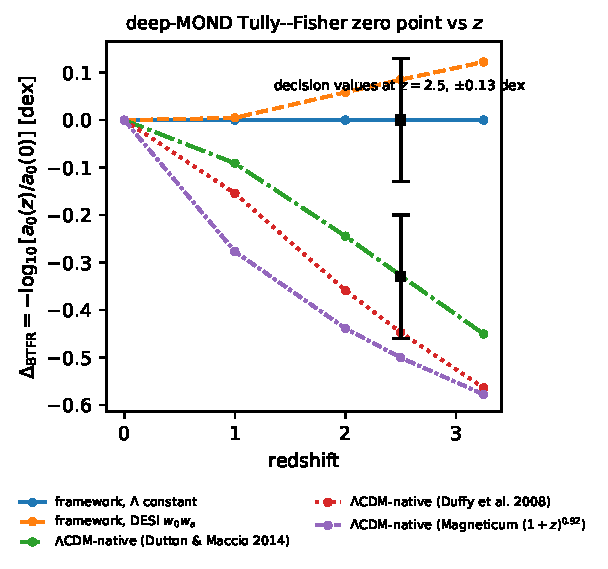
\includegraphics[width=\columnwidth]{fig4_a0z.pdf}
\caption{The deep-MOND Tully--Fisher zero point against redshift for the framework's law (flat, and the DESI $w_0w_a$ decline) and three $\Lambda$CDM-native scalings of the emergent acceleration scale. The two black points at $z=2.5$ show the pre-registered decision values, $0.00$ and $+0.33$ dex, each with the required $\pm0.13$ dex. Values from \texttt{a0z\_lcdm\_native\_hypothesis\_2026.py}.}
\label{fig:a0z}
\end{figure}

\section{Discussion}
The relation of equation~(\ref{eq:relation}) is not new and its derivation attempts have prior art; what this paper adds is a precise statement of what is and is not fixed. (i) Within the aether--scalar class of local actions the coefficient cannot be forced: the zero of the MOND primitive is a zero mode, the sign of any vacuum energy the scalar can supply is wrong, and the two repairs that could fix the zero fail. (ii) A four-form promotion of $a_0$ turns the form of the relation into structure and the coefficient into a coupling ratio $Z/\beta^2=8$, with a testable side effect in the innermost wide-binary bin. (iii) On the observational side the coefficient is not a rational number the data pick out; it is a value with a 10--16 per cent error, an irreducible $H_0$-convention dependence, and an exact degeneracy with the Hubble tension between the two coefficient candidates that survive. (iv) The two observations that move the question are registered before the data.

Three limitations should be stated. The theorem concerns local actions of one class; a principle acting in the geometric or boundary sector, of the type the horizon coefficient gestures at, is not excluded and is where a derivation would have to live. The candidate action's dark sector is not part of this paper: on the programme's own record no condensate or particle completion tested so far survives its cluster and galaxy gates simultaneously, and the tests registered here are coefficient-blind and independent of that question. And the wide-binary Arm B is, as a prediction, one-sided: DR4 can kill it from above but cannot confirm it at the frozen sample size; confirmation needs roughly four times the sample or a different observable.

\section{Conclusions}
The coefficient $\kappa$ in $a_0=\kappa c\sqrt{G\rho_\Lambda}$ is measured to be $0.45$--$0.59$ depending on estimator and $H_0$ convention, is not derived by any local MOND action of the aether--scalar class, and cannot be separated from the horizon coefficient 0.461 by present data, with which it is exactly degenerate through $H_0$. A four-form construction fixes the sign of the vacuum energy and makes $a_0\propto\sqrt{G\rho_\Lambda}$ structural at the price of one free coupling ratio. Two pre-registered tests, the Gaia DR4 wide-binary boost with two mutually exclusive arms and the deep-MOND Tully--Fisher zero point of a lensed rotator at $z\simeq2.5$, are the observations that decide the redshift dependence of the scale and the survival of the covariant candidate; the coefficient itself waits on a stellar mass-to-light zero point, an absolute gas scale and a settled $H_0$.

\section*{Acknowledgements}
The derivations, code and drafting in this work were carried out with the assistance of large language models (Anthropic Claude and OpenAI models) operated by the author; every derivation was executed as a committed script with checks that can fail, and the author reviewed and takes full responsibility for the content. The four-form construction of Section~\ref{sec:fourform} and the observing-funnel ordering of Section~\ref{sec:a0z} were proposed in exchanges with an OpenAI model and audited here. This work made use of the SPARC database \citep{Lelli2016} and the Gaia EDR3 wide-binary catalogue of \citet{ElBadry2021}.

\section*{Data Availability}
All scripts, outputs and pre-registration documents are in the public repository at \url{https://github.com/carlzimmerman/zimmerman-formula}: the coefficient audit in \texttt{kappa\_closure/} (\texttt{k01}--\texttt{k04}), the estimators in \texttt{real\_research/reviews/} (\texttt{mi\_btfr\_intercept\_kappa\_door\_2026.py}, \texttt{mi\_distance\_free\_gbar\_estimator\_sparc\_2026.py}, \texttt{kappa\_h0\_convention\_audit\_2026.py}), the wide-binary pipeline and pre-registration with its hash-stamped amendments in \texttt{prep\_2026/gaia\_dr4\_prep/}, the high-redshift likelihood and target ledger in \texttt{prep\_2026/a0z\_crossscale/}, and the figure script of this paper in \texttt{qwen\_claude\_field\_theory/papers\_2026/mnras\_submission\_2026/}. Deposited versions: \citet{Zimmerman2026kappa,Zimmerman2026a0z,Zimmerman2026prereg}. SPARC is public; the El-Badry catalogue is at Zenodo record 4435257.

\bibliographystyle{mnras}
\bibliography{references}

\bsp
\label{lastpage}
\end{document}
